\documentclass[a4paper,12pt]{article}
\usepackage{graphicx} % For including images
\usepackage{caption}  % For custom captions
\usepackage{float}    % For forcing figure placement

\title{Lab 5: Operating System}
\author{Muhammad Shafeen \\ Roll No: 22P-9278}
\date{\today}

\begin{document}

\maketitle

\section*{Lab Task :}

\section{Commands and Outputs}
\subsection{Command: \texttt{ls -lh}}
Gives details of the file about permissions.
\begin{center}
    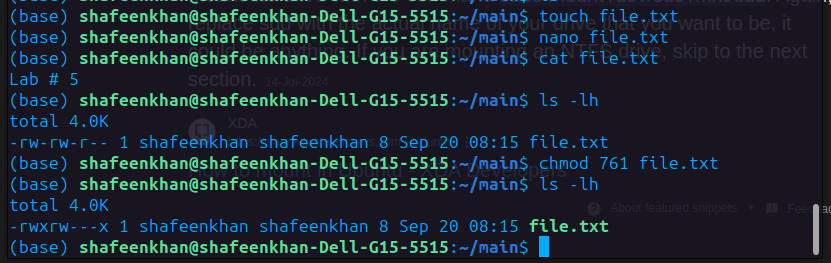
\includegraphics[width=\linewidth]{Screenshot from 2024-09-20 08-19-19.png}
\end{center}

\subsection{Command: \texttt{chmod 000 file.txt}}
The command is used to give permission to the file.
\begin{center}
    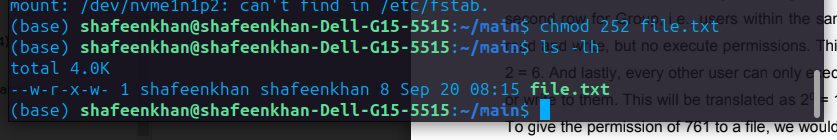
\includegraphics[width=\linewidth]{Screenshot from 2024-09-20 08-31-20.png}
\end{center}

\subsection{Command: \texttt{Question : --w-r-x-w-}}
Changed the permission to the above by calculating and then doing chmod 746
\begin{center}
    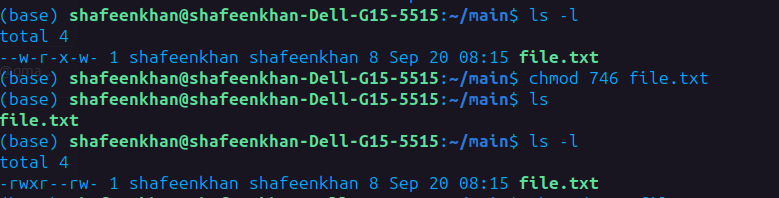
\includegraphics[width=\linewidth]{Screenshot from 2024-09-20 08-55-46.png}
\end{center}

\subsection{Command: \texttt{chmod o+x file.txt}}
Giving the file execute command for others 
\begin{center}
    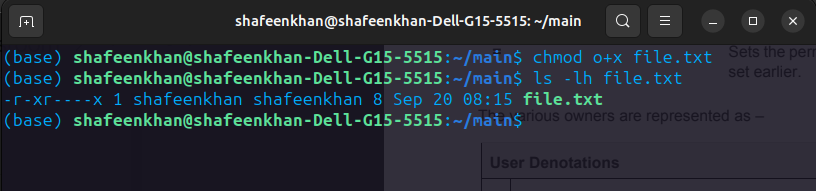
\includegraphics[width=\linewidth]{Screenshot from 2024-09-20 08-57-44.png}
\end{center}

\subsection{Command: \texttt{chmod o+w file.txt}}
Giving the file write command for others 
\begin{center}
    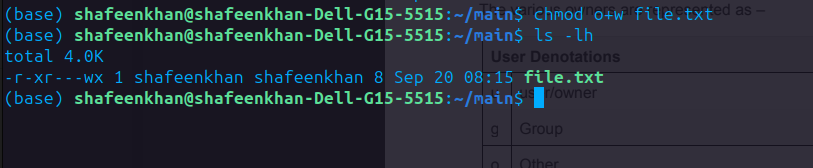
\includegraphics[width=\linewidth]{Screenshot from 2024-09-20 08-59-03.png}
\end{center}

\subsection{Command: \texttt{chmod 000 file.txt}}
take all permissions from other user
\begin{center}
    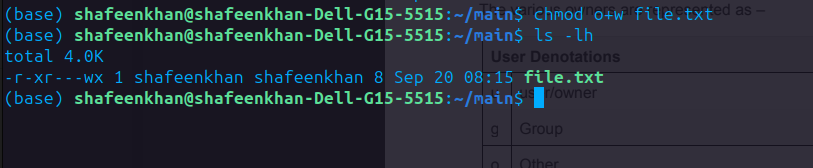
\includegraphics[width=\linewidth]{Screenshot from 2024-09-20 08-59-03.png}
\end{center}

\subsection{Command: \texttt{chmod o+rwx file.txt}}
Giving permissions to others with symbolic commands
\begin{center}
    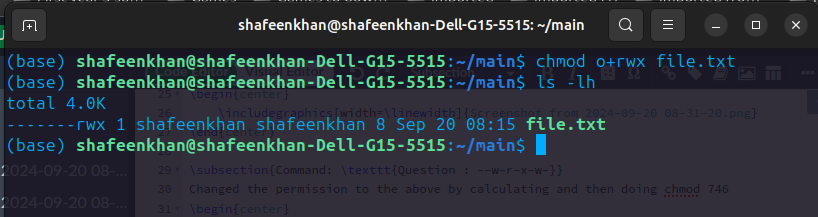
\includegraphics[width=\linewidth]{Screenshot from 2024-09-20 09-02-42.png}
\end{center}


\subsection{Command: \texttt{Give --w-r-x-w- with symbolics}}
Giving --w-r-x-w- permissions to others with symbolic commands
\begin{center}
    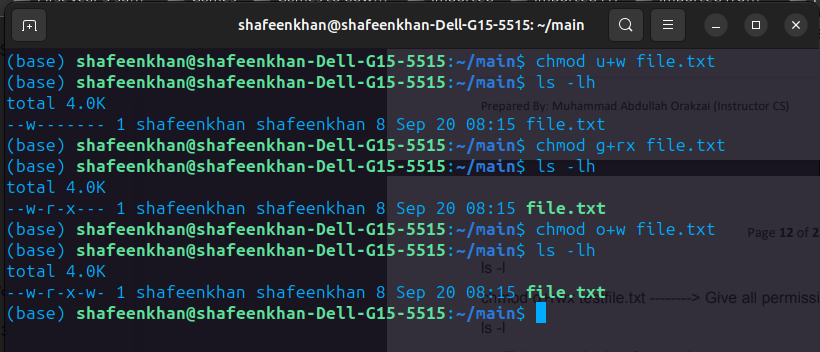
\includegraphics[width=\linewidth]{image.png}
\end{center}

\subsection{Command: \texttt{Give --w-r-x-w- with symbolics in one line }}
Giving --w-r-x-w- permissions to others with symbolic commands
\begin{center}
    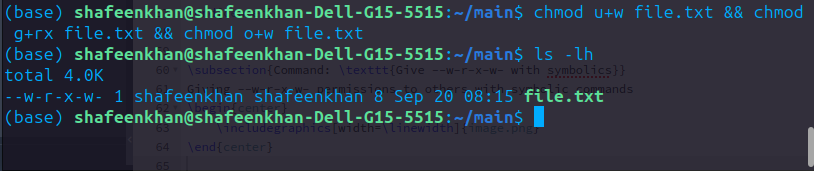
\includegraphics[width=\linewidth]{Screenshot from 2024-09-20 09-13-53.png}
\end{center}


\subsection{Command: \texttt{chmod ug=rwx file.txt}}
Give all permissions to user and group
\begin{center}
    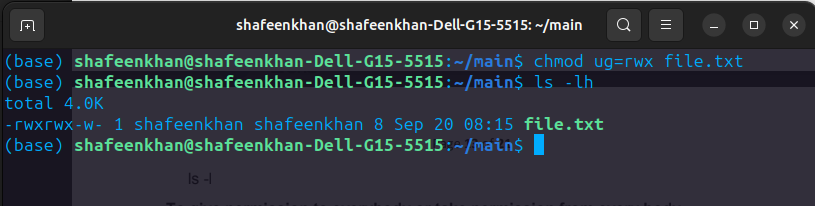
\includegraphics[width=\linewidth]{Screenshot from 2024-09-20 09-15-11.png}
\end{center}

\subsection{Command: \texttt{chmod ugo=rwx testfile.txt}}
give all permissins to everyone , owner , group , user
\begin{center}
    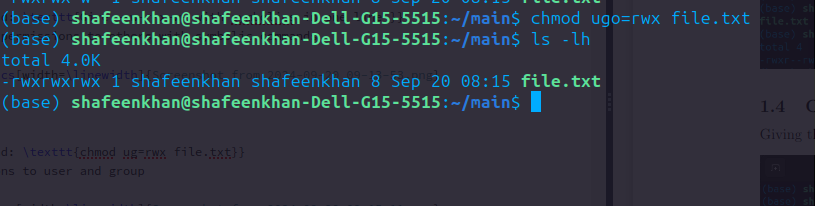
\includegraphics[width=\linewidth]{Screenshot from 2024-09-20 09-16-52.png}
\end{center}

\subsection{Command: \texttt{chmod ugo+rwx file.txt}}
Give all permissions to everyone 
\begin{center}
    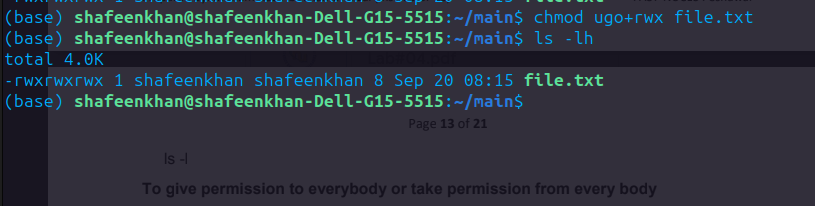
\includegraphics[width=\linewidth]{Screenshot from 2024-09-20 09-17-56.png}
\end{center}

\subsection{Command: \texttt{chmod ugo-rwx file.txt}}
Take all permissions to everyone 
\begin{center}
    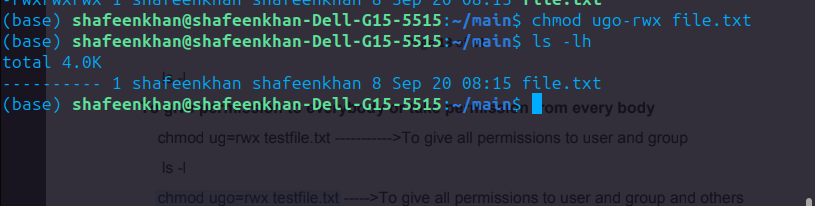
\includegraphics[width=\linewidth]{Screenshot from 2024-09-20 09-18-13.png}
\end{center}

\subsection{Command: \texttt{chmod u+w file.txt}}
Give user write commands
\begin{center}
    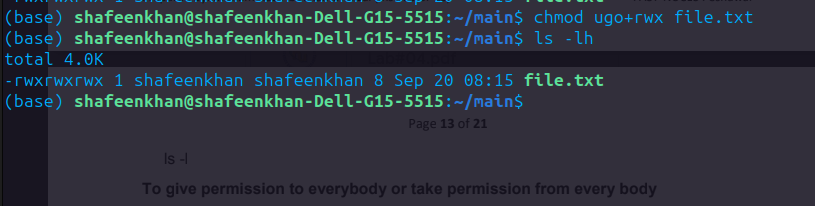
\includegraphics[width=\linewidth]{Screenshot from 2024-09-20 09-17-56.png}
\end{center}

\subsection{Command: \texttt{chmod u-w file.txt}}
Take write command from user
\begin{center}
    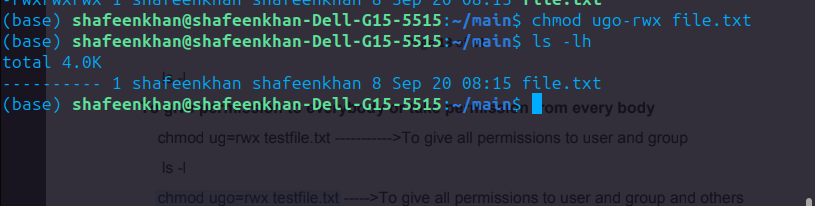
\includegraphics[width=\linewidth]{Screenshot from 2024-09-20 09-18-13.png}
\end{center}

\subsection{Command: \texttt{chmod a+wrx file.txt}}
give all command to user
\begin{center}
    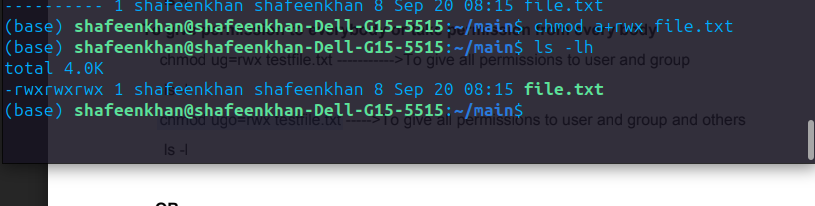
\includegraphics[width=\linewidth]{Screenshot from 2024-09-20 09-18-24.png}
\end{center}

\subsection{Command: \texttt{chmod a-wrx file.txt}}
Take all command from user
\begin{center}
    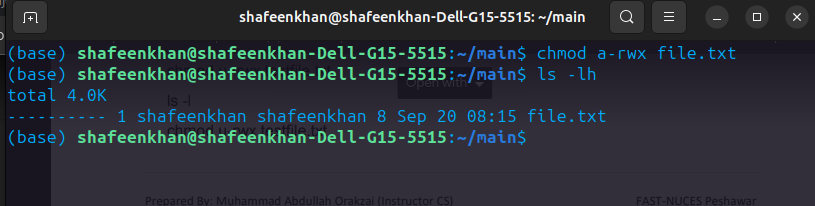
\includegraphics[width=\linewidth]{Screenshot from 2024-09-20 09-18-50.png}
\end{center}

\subsection{Command: \texttt{chmod a-rwx abc/}}
Take all permission from directory
and try to access it
\begin{center}
    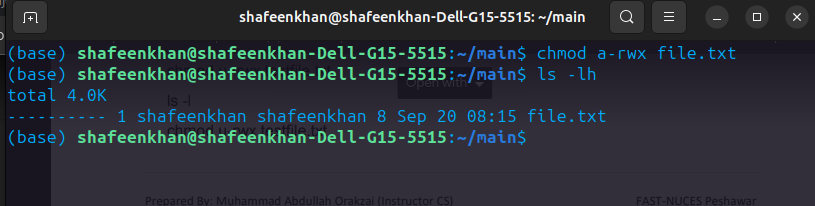
\includegraphics[width=\linewidth]{Screenshot from 2024-09-20 09-18-50.png}
\end{center}

\subsection{Command: \texttt{Give execute command to abc and try to write}}
Give execute command and try to view files in abc and write something in it
\begin{center}
    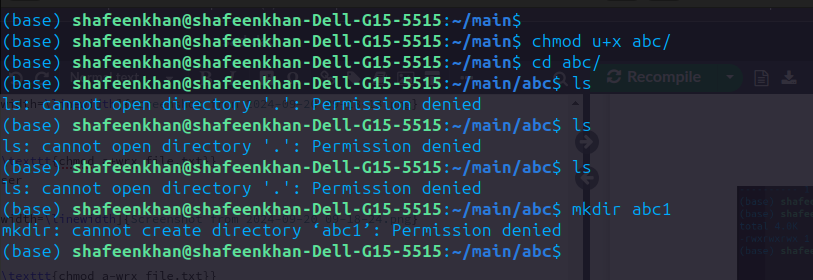
\includegraphics[width=\linewidth]{Screenshot from 2024-09-20 09-46-51.png}
\end{center}

\subsection{Command: \texttt{chmod u+w abc , touch file}}
Create file in abc directory and try to access it wont
\begin{center}
    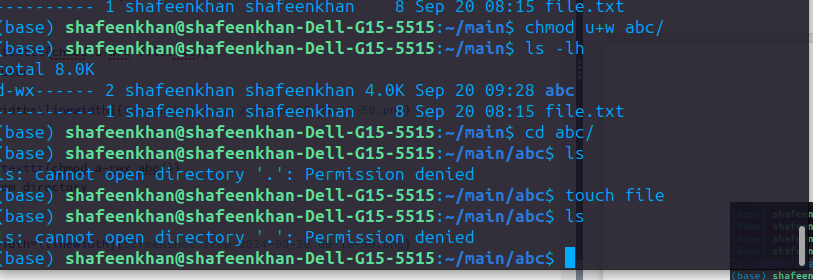
\includegraphics[width=\linewidth]{Screenshot from 2024-09-20 09-51-09.png}
\end{center}

\subsection{Command: \texttt{Make directory abc1 \\ and make text file in it}}
\begin{center}
    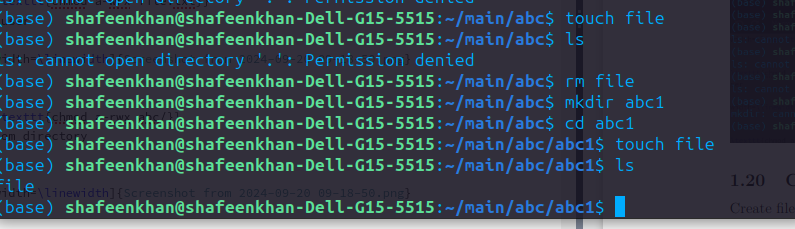
\includegraphics[width=\linewidth]{Screenshot from 2024-09-20 09-52-39.png}
\end{center}

\subsection{Command: \texttt{Give read permission- \\to abc and then check}}
\begin{center}
    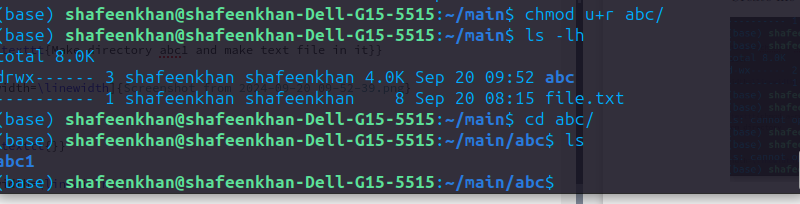
\includegraphics[width=\linewidth]{Screenshot from 2024-09-20 09-56-22.png}
\end{center}

\subsection{Command: \texttt{Give all permission- \\to abc's group and then check}}
\begin{center}
    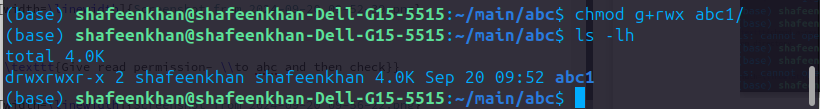
\includegraphics[width=\linewidth]{Screenshot from 2024-09-20 09-59-23.png}
\end{center}

\subsection{Command: \texttt{Give all permission- \\to abc's other and then check}}
\begin{center}
    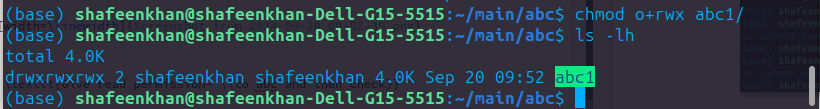
\includegraphics[width=\linewidth]{Screenshot from 2024-09-20 10-00-11.png}
\end{center}

\subsection{Command: \texttt{Take all permission- \\from abc's user and then check}}
\begin{center}
    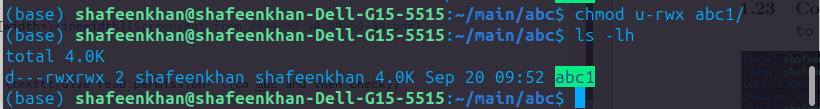
\includegraphics[width=\linewidth]{Screenshot from 2024-09-20 10-01-19.png}
\end{center}

\subsection{Command: \texttt{chown root file.txt \\, sudo chown root file.txt}}
changed the owner of file.txt from shafeenkhan to root
\begin{center}
    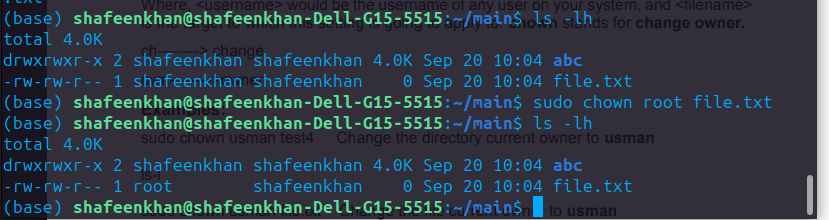
\includegraphics[width=\linewidth]{Screenshot from 2024-09-20 10-07-54.png}
\end{center}

\subsection{Command: \texttt{Changing user to root}}
changed the owner of abc from shafeenkhan to root
\begin{center}
    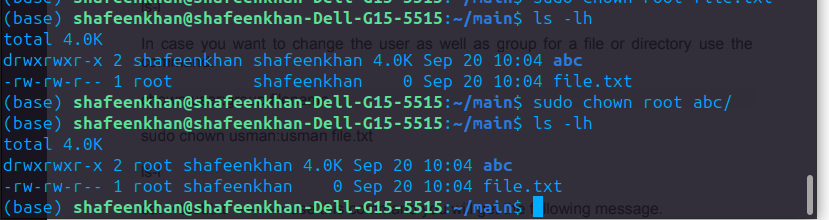
\includegraphics[width=\linewidth]{Screenshot from 2024-09-20 10-11-34.png}
\end{center}


\subsection{Command: \texttt{changing group to root as well}}
changed the group of abc from shafeenkhan to root
\begin{center}
    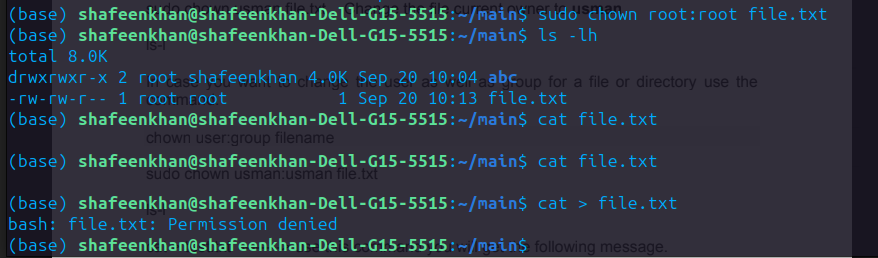
\includegraphics[width=\linewidth]{Screenshot from 2024-09-20 10-15-27.png}
\end{center}

\subsection{Command: \texttt{nano hello.c ,\\ gcc hello.c , ./a.out}}
Making a c file and then running a simple hello world command
\begin{center}
    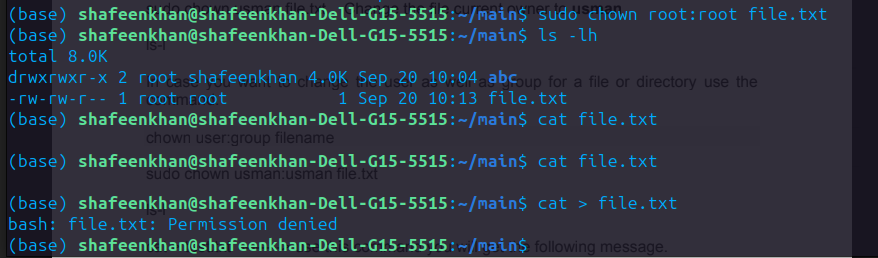
\includegraphics[width=\linewidth]{Screenshot from 2024-09-20 10-15-27.png}
\end{center}

\subsection{Command: \texttt{nano hello.c ,\\ gcc hello.c , ./a.out}}
using the system("ls -l");
\begin{center}
    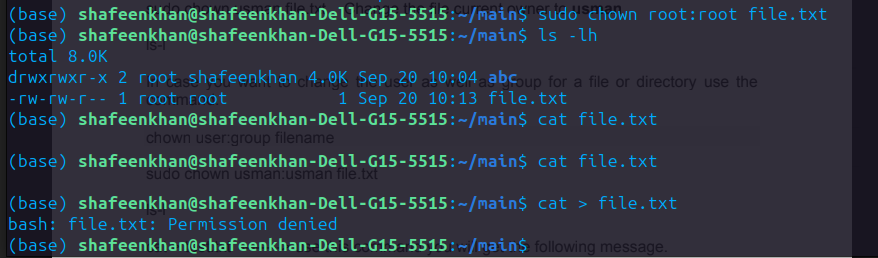
\includegraphics[width=\linewidth]{Screenshot from 2024-09-20 10-15-27.png}
\end{center}

\end{document}
